\begin{chapter}{Resultados}
\label{cap4}

\hspace{5 mm} Nesse cap�tulo discutiremos sobre os resultados obtidos nas simula��es descritas no cap�tulo anterior. Resultados obtidos de m�todos alternativos s�o usados como compara��o e valida��o.

\section{Transfer�ncia de momento angular}

\hspace{5 mm}Primeiramente, devemos observar que o efeito de torque negativo � dependente de aberra��es �ticas. O astigmatismo desempenha um papel de atenuar esse efeito, podendo at� trocar o sinal de $\kappa_\phi$\cite{Diniz2019}. No nosso caso, os �ngulos de rota��o da microesfera ao redor da posi��o de equil�brio ($\phi$) s�o simplesmente diminu�dos. Isso nos possibilita tentar ajustar uma curva simulada com o modelo MDSA+ com o par�metro de astigmatismo $A_{ast}$ como vari�vel livre. 

Usamos um m�todo de m�nimos quadrados para realizar esse ajuste. Dado o conjunto de pontos experimentais $\phi_i^{exp}$, calculamos a fun��o erro $E$ do conjunto de pontos simulados $\phi_i^{sim}$, onde cada �ndice $i$ corresponde a um �ngulo $\psi$ na placa de quarto de onda. A fun��o erro � definida como:
%
\begin{equation}
E(A_{ast})=\sum \limits_i \big{[} \phi_i^{exp} - \phi_i^{sim}(A_{ast}) \big{]}^2.
\label{erro}
\end{equation}

A figura \ref{alpha_0} mostra o conjunto de pontos experimentais (em vermelho) e os pontos para a teoria MDSA sem astigmatismo (em azul). 
%
\begin{figure}
\begin{center}
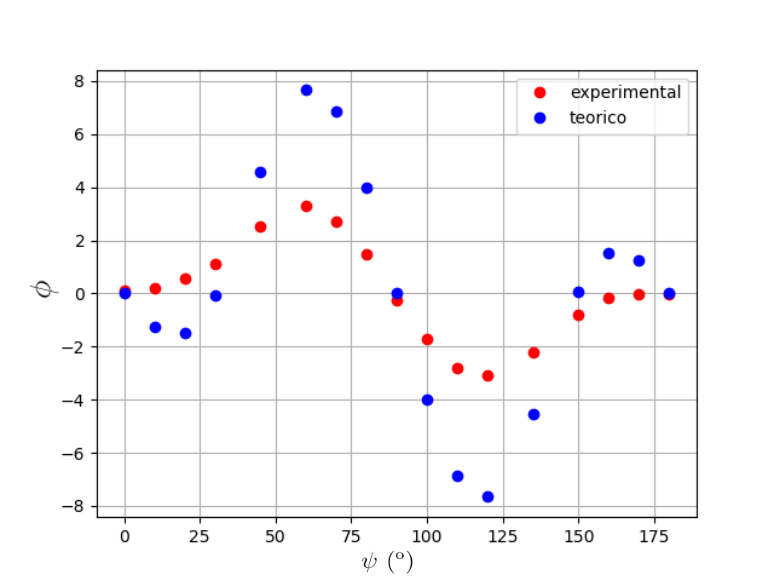
\includegraphics[scale=.8]{Kphi_rho_Aast0II}
\caption{}
\label{alpha_0}
\end{center}
\end{figure}
%


%
\begin{figure}
\begin{center}
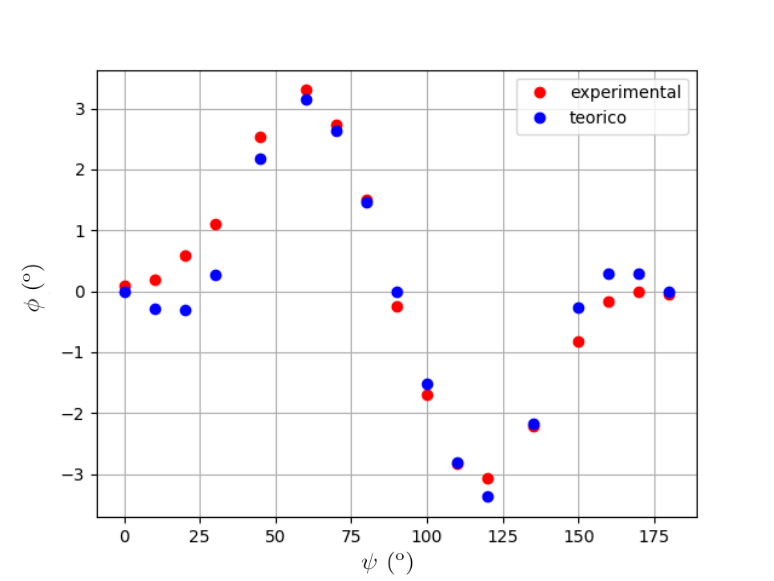
\includegraphics[scale=.8]{Kphi_rho_Aast024II}
\caption{}
\label{alpha_024}
\end{center}
\end{figure}
%

Podemos ver que as contribui��es mais importante para o ajuste s�o os pontos em volta dos �ngulos $60�$ e $120�$.


\end{chapter}
